\chapter[Problemas Encontrados]{Problemas Encontrados}

Esta seção tem como foco a explicação dos problemas encarados e das soluções adaptadas, durante o desenvolvimento do projeto. Tanto como grupo quanto em subdivisões especificas feitas.

 \subsection{Geral}

-Dificuldade na definição das atividades da Sprint: No início do projeto foi definido que nossa organização seria baseada na metodologia ágil, sendo assim teríamos tarefas semanais.
    \begin{itemize}
      \item Problema: De uma forma geral, o grupo superestimou as atividades nas sprints, tornando muito difícil a conclusão das atividades propostas para a sprint.
	  \item Solução: Como solução granularizamos as atividades reduzindo-as para que fosse possível realizá-las no tempo de uma sprint e durante a mudança, que durou cerca de 3 sprints, calibramos os erros e acertos na retrospectiva feita ao final de cada sprint
.

    \end{itemize}

-Redistribuição do pessoal da área de Power Train para a área de Controle e Estrutura, porque as atividades propostas para a área de Power Train foram concluídas. Baseado nisso foi feita a escolha de realocar os componentes desta área para a área de Controle.
    \begin{itemize}
      \item Problema: Realocar os componentes de forma a não ficarem ocioso em alguma atividade.
	  \item Solução:Relocar os componentes conforme maior expertise dos mesmos na área de Controle e Estrutura.

    \end{itemize}

-Gastos com materiais
    \begin{itemize}
  \item Problema: Na fase inicial do trabalho muitas pesquisas foram feitas e os materiais necessários levantados, porém não era de conhecimento o quanto gastaríamos com o projeto.
  \item Solução: Desde o inicio já começamos a arrecadar dinheiro dos integrantes e com o amadurecimento do projeto conseguimos mensurar de forma mais real qual seria o custo do projeto sendo possível assim um planejamento financeiro melhor.

    \end{itemize}

\subsection{Controle}

-LINGUAGEM NOVA: Mesmo com a experiência do grupo dos alunos de software, houve problemas em relação ao Phyton, como: entendimento da exportação relativa de classes em outras pastas, mudança da versão 2.7 para a versão 3.4 e problemas de identação relacionado a IDE de desenvolvimento.
1 Ambiente de desenvolvimento:

-Testes unitários do código-fonte.
    \begin{itemize}
      \item Problema: Utilização do framework de teste de forma correta.
	  \item Solução: Olhar a documentação do framework e aprender como utilizar.

    \end{itemize}

-Mock
 \begin{itemize}
      \item Problema: Entendimento de como utilizar o "Mock" para fingir que o Hardware existe.
	  \item Solução: Conversa entre grupos da disciplina de Projeto Integrador 2 e leitura e compreensão da documentação.

    \end{itemize}

-Cobertura de código em Python
 \begin{itemize}
      \item Problema: Como fazer cobertura de código para Python.
	  \item Solução: Depois de realizar pesquisas o Coverage foi escolhido e instalado inicialmente no repositório local para teste e depois que confirmada a eficiencia foi instalado na Raspberry Pi.
    \end{itemize}

2 Ambiente físico: O ambiente físico utilizado para desenvolvimento do software deste projeto é um Raspeberry Pi, vide seção 2.2.2.1, referente as configurações do mesmo.
-SSH
 \begin{itemize}
      \item Problema:  O acesso via SSH é feito através de um cabo de rede, no qual somete uma máquina por vez pode acessar. Isso ocasiona um problema de ociosidade na equipe: enquanto um componente o utiliza, os outros 2 ficam ociosos.
	  \item Solução: Utilizar o Raspeberry conectado a um roteador Wi-Fi, que permite a todos os integrantes utilizarem do ambiente mutualmente via rede sem fio.
    \end{itemize}

-Mudança de Sistema Operacional: Pode ser instalado no Raspberry um sistema operacional que possibilite a facilidade de uso, mediante as necessidades de quem o instala.
 \begin{itemize}
      \item Problema:  Problema relacionado: Pretende-se utilizar um ambiente para teste que possibilite o desenvolvimento de forma completa mediante o possível para o projeto. Para isto é necessário o uso de testes unitários e do "Mock", descobriu-se que o primeiro SIstema Operacional instalado (Raspdebian Wheezy) não atende para a utilização do "Mock".

	  \item Solução:Um outro Sistema Operacional foi instalado (Raspdebian Jessie), por possuir nativamente um ambiente de testes robusto que possibilite o uso de testes unitários e "Mock".
    \end{itemize}

-Quantidade de MSPs a serem utilizados: A utilização de vários MSPs é uma ótima alternativa para separar componentes independentes e utilizar ferramentas como conversor AD, gerador de PWM e temporizador de forma simples, barata e rápida.
 \begin{itemize}
      \item Problema: Unificar todo o controle no Raspberry Pi diminui a confiabilidade do sistema, além disso, ele não tem conversores analógico/digital, necessários para o sistema de controle.

	  \item Solução: MSPs dedicados a cada componente foram utilizados, por sua facilidade em implementar conversores AD de vários canais, PWMs e por ser de fácil comunicação com o Raspberry Pi via serial UART.

    \end{itemize}

- Arquitetura
 \begin{itemize}
      \item Problema: Esta arquitetura possui 2 formas de serem montadas: Paralela ou Sequêncial. A Paralela nos permite ter várias "threads" acontecendo simultaneamente para difererentes situações. A Sequêncial acontece de forma sucessiva em somente uma  "thread". Houve a dúvida técnica de qual destas implementar em tempo de apresentação do produto. Existiu o temor de não se obter uma Arquitetura, caso fosse usado a solução Paralela.

	  \item Solução 1: Foi sugerido que uma montagem da solução sequêncial fosse montada para se fazer uma avaliação, em relação ao tempo de resposta que seria entre o usuário fazer o movimento com o Joystick e o motor responder ao movimento.
  \item Solução 2: Foi sugerido que a contabilização do tempo de execução (delay dos compontentes eletrônicos + complexidade do software) fosse feita, para analisar e ter certeza de que a solução Sequêncial diferenciaria muito da solução Paralela.

    \end{itemize}

-Simulações da Ponte H
 \begin{itemize}
      \item Problema:Se colocado alto nível nas duas entradas o motor poderia “explodir”.

	  \item Solução:Colocar uma porta lógica no início para corrigir essa falha, assim quando a ponte H receber nível lógico nas duas entradas o motor não responderá

    \end{itemize}

-Joystick
 \begin{itemize}
  \item Problema: Inicialmente utilizamos um joystick de um controle de videogame (PlayStation 2). Este não se adequou às nossas necessidades.
  \item Solução: Adquirimos um joystick que tivesse conectores, facilitando assim a prototipagem e implementação. Ainda estamos aguardando sua chegada para verificar se esse joystick se adequaria.

 \end{itemize}

\subsection{Power Train}

-Escolha de um motor que atendesse os requisitos velocidade-torque.
 \begin{itemize}
  \item Problema: A escolha do melhor método de cálculo de potência necessária para mover o sistema completo (cadeira de rodas mais usuário) foi um problema devida a alta variedade de possibilidades, tornando-se muito indecisa a precisão dos cálculos.
  \item Solução: Após uma vasta pesquisa na literatura e com alguns professores da FGA, com o auxilio do software Matlab, foram feitas diversas simulações envolvendo as variáveis de projeto para a decisão do melhor conjunto.

  \item Problema: Motores de corrente contínua fornecem um baixo torque, através dos cálculos, observou-se que era preciso um torque alto.
  \item Solução: Foi necessário o uso de um redutor para atender as especificações matemáticas do projeto. A partir disso foi feita uma busca de mercado e optamos por encomendar um kit motor-redutor pronto

 \end{itemize}

-Eixo do conjunto moto-redutor
 \begin{itemize}
  \item Problema: Os primeiros conjuntos moto-redutor que foram analisados foram o de motor de para-brisas de carro, esses conjuntos não forneciam a velocidade especificada pelo projeto, porém foram úteis para testes de controle. E seria fácil acoplar a roda do sistema a esse conjunto devido ao seu design. Entre tudo, quando os motores reais do projeto chegaram, o eixo era muito curto e devido ao design seria impossível conectar diretamente as rodas
  \item Solução: Será necessário fazer um novo eixo com o uso do torno mecânico para ligar a roda ao conjunto moto-redutor.

 \end{itemize}

\subsection{Estrutura}
-Acoplamento
 \begin{itemize}
  \item Problema: O ponto mais importante a se considerar para que o projeto funcione de modo eficaz e robusta é a forma como o sistema se acopla a cadeira, pois o deslocamento sera feito através da rotação das rodas acopladas a mala, ou seja, caso  a conexão não fique firme o deslocamento sera comprometido.
  \item Solução 1: Primeiramente se pensou em criar um sistema de garras que seriam presas a estrutura tubular da cadeira, o que seria eficaz e simples de ser feito, porem após conseguir cadeiras reais para análise foi constatado que não haveria como acoplar as garras a algumas cadeiras devido a forma como os fabricantes fixam o tecido que mantem o encosto para as costas no lugar. Então foi pensado em utilizar velcros que seriam baratos, fáceis de utilizar e se bem posicionados permitiriam uma boa fixação, m...(line truncated)...
  \item Solução 2: Em seguida foi pensado em uma forma de acoplamento que não fosse afetada por diferentes tipos de modos de montagem ou disposição de partes da cadeira. Tendo em mãos duas cadeiras de rodas reais e distintas notou se a presença de dois pontos livres para realizar o acoplamento. Com a solução em mente foi decidido criar um protótipo em PVC, devido ao baixo custo, para que fosse possível analisar de fato se o sistema de acoplamento idealizado seria eficaz. Apos construída a estrutura foi const...(line truncated)...

 \end{itemize}

-Falta de cadeira
 \begin{itemize}
  \item Problema: Não se tinha cadeiras de rodas disponíveis para teste da estrutura.
  \item Solução: Entramos em contato com os professores responsáveis pela cadeira de rodas presente no laboratório e conseguimos autorização para utilizá-la. Outras cadeiras foram conseguidas por meio de doações de terceiros.

 \end{itemize}

\chapter[Perspectiva]{Perspectiva}

\section{Incremento atual}
  \subsection{Estrutura}
    \begin{enumerate}
      \item Modelagem da cadeira motorizada adaptada: Foi feito a modelagem da cadeira de rodas levando em conta a solução de portabilidade e acessibilidade da mesma, pontuando pontos como o design de inovação do anexo autômato a cadeira;

      \item Escolha do material a ser usado em anexo: Um estudo dos possíveis materiais será realizado, alavancando os motivos e vantagens do uso dos mesmos para suporte das cargas;

      \item Ergonomia do produto: Estudo e modelagem do melhor design da cadeira de rodas manual com o anexo que a motoriza;

 \item Desenvolvimento de um modelo de PVC para testes do sistema de acoplamento;

 \item Desenvolvimento do eixo que ira transmitir potência entre a roda ao conjunto de moto-redução.

    \end{enumerate}
  \subsection{Power Train}
    \begin{enumerate}
      \item Escolha do motor elétrico quanto ao custo do mesmo no projeto, embasado em estudo feito em relação a peso, velocidade máxima, velocidade nominal;
      \item Especificação do motor elétrico de Corrente Contínua quanto a potência minima;
      \item Estudo e especificação sobre baterias a serem utilizadas, quanto tensão, capacidade e dimensão. Foi escolhido usar as baterias de Chumbo-Ácida selada, levanto em conta vantagens e limitações. Os cálculos de autonomia foram feitos para melhor estimar o método de carregamento da bateria;

 	\item Estudo com o auxílio do software Matlab da interferência da roda e do peso do sistema no desempenho do conjunto de moto-redução;
 	\item Foram adquirido dois conjuntos de moto-redução  pela empresa MKS Redutores de São Paulo. O motor com redutor escolhido para o projeto foi o MR com motor GPB que possui as seguintes especificações com potência de 305 a 350 W e redução de 1:10.

    \end{enumerate}

    \subsection{Controle}
      \begin{enumerate}
        \item Especificação de tecnologia: Estudo e escolha da melhor tecnologia voltada para o problema, que no caso será feito com um Raspberry Pi para comunicação entre a interface do usuário e o motor;

        \item Controle de potência: Estudo de qual tipo de controlador de potência a ser usado no motor, para controle de sua corrente. A escolha da utilização da ponte H será combinado com o algoritmo de PWM, que utiliza o Raspberry Pi como forma de resposta aos comandos dos usuários como a diração, aceleração, frenagem da cadeira motorizada adaptada;

        \item Escolha da linguagem de programação: Definição de qual linguagem será utilizada com base na problemática existente e nos recursos a serem utilizados. A linguagem escolhida foi o Phyton, pois existem bibliotecas especificas que controlam GPIO do Raspebery Pi.

      \end{enumerate}

  \subsection{Interface com Usuário}
    \begin{enumerate}
      \item Estudo de tecnologias para interfaces: Estudo de quais tecnologias são usadas como interface de usuário para controle da cadeira motorizada adaptada. Neste estudo são observados dispositivos de controle como Joystick e aplicativos que podem utilizar tecnologia Bluetooth ou VPN para comunicar com o Raspberry Pi.

      \item Escolha da linguagem de programação do aplicativo: Definição de qual linguagem será utilizada com base na problemática existente e nos recursos a serem utilizados. A linguagem escolhida para o desenvolvimento do aplicativo será definida conforme o resultado de estudo de utilziação de Bluetooth e VPN. Caso a escolha seja para dispositivos Android, então pode ser escolhida a linguagem nativa Java, caso a escolha seja para dispositivos iOS, então pode ser escolhida a linguagem nativa Objective-C ou Swift.

    \end{enumerate}

\section{Próximos passos}
  \subsection{Estrutura}
    \begin{enumerate}
      \item Testes com o eixo acoplado ao motor;
      \item Escolha de material mediante norma ABNT 6061 - T6;
	 \item Desenvolvimento do protótipo.
    \end{enumerate}
  \subsection{Power Train}
    \begin{enumerate}
      \item Testes em conjunto com a parte de estrutura e controle.
      \end{enumerate}

  \subsection{Interface com Usuário}
    \begin{enumerate}
      \item Montagem do Joystick ergonômico.

    \end{enumerate}
  \subsection{Controle}
    \begin{enumerate}
     \item Implementação de filtro para suavizar movimentos do Joystick para motores;
     \item Implementação dos testes para os códigos do MSP;
     \item Implementação dos sensores de nível de bateria e velocidade em MSP;
    \end{enumerate}

\section{Cronograma}

  Para prosseguir com os próximos passos um cronograma com as estimativas de cada Sprint foi levantado.

  \begin{figure}[!htb]
  \centering
    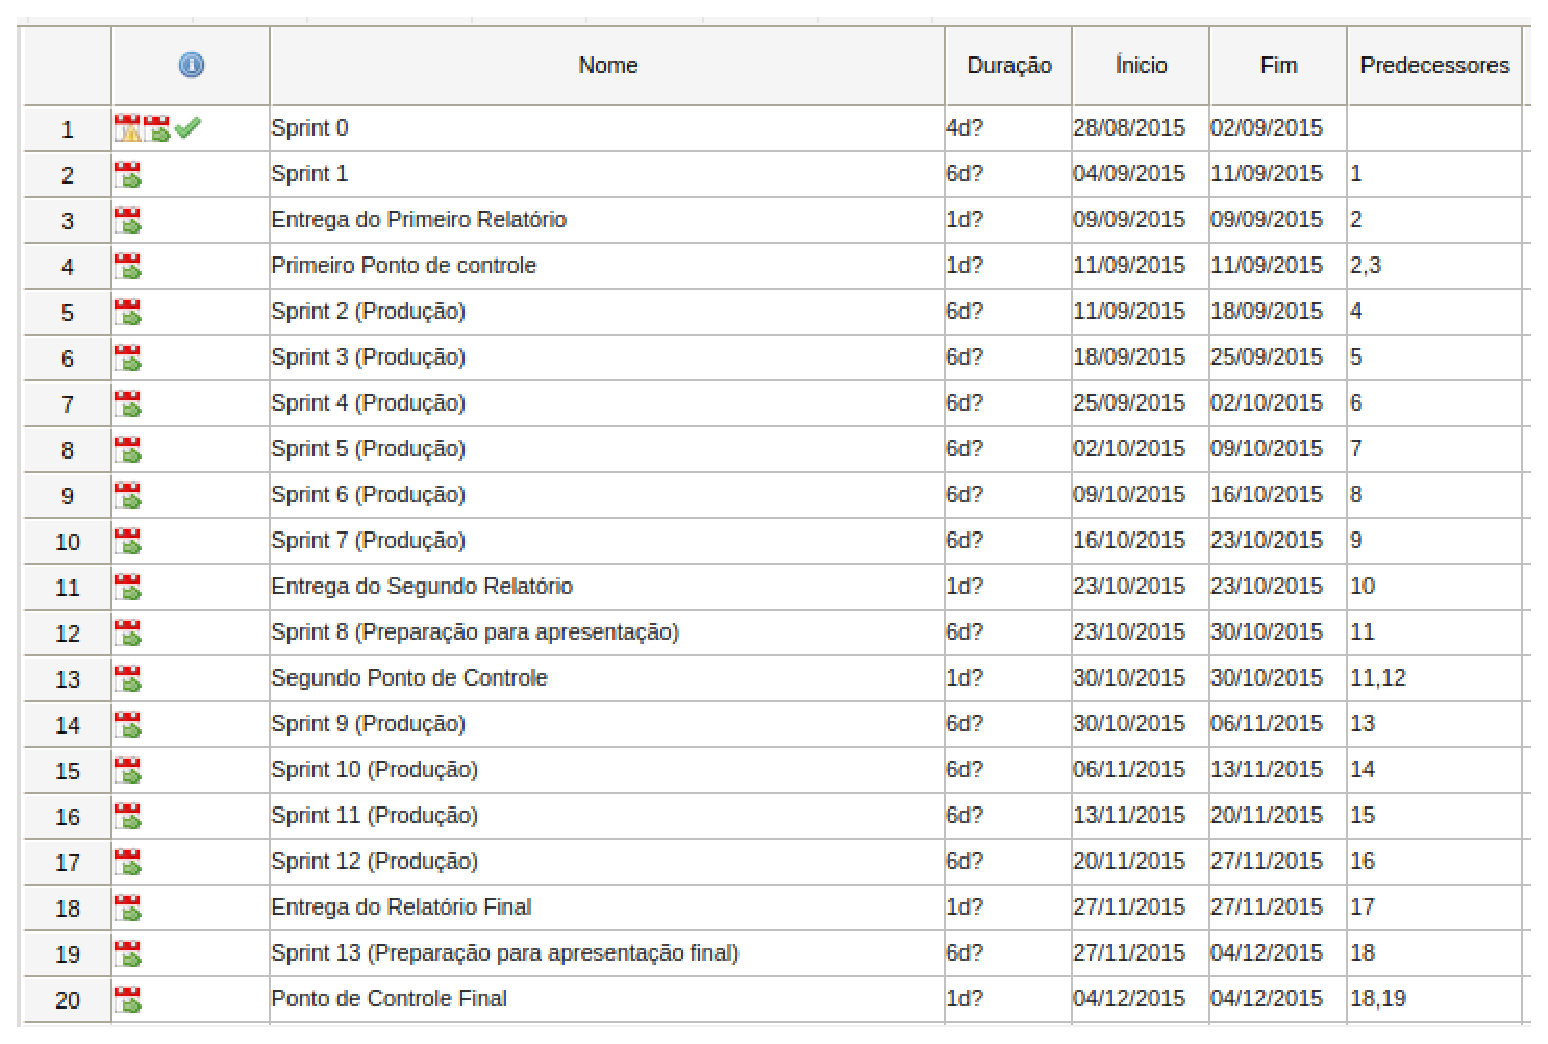
\includegraphics[keepaspectratio=true,scale=0.5]{figuras/metodologia/cronograma}
  \caption{Cronograma}
  \label{fig:cronograma}
  \end{figure}
